\subsection{Optimisation of Transformer Networks}
\label{subsec:Optimisation of Transformer Networks}
\citet{wu2020lite} pointed out that even though Transformer-based models achieve state-of-the-art results in natural language processing tasks ubiquitously, it is unsuitable for running on mobile devices because the self-attention mechanism puts a lot of pressure on storage and computation.
To tackle the problem, \citet{wu2020lite} proposed a Lite Transformer model that uses Long-Short Range Attention (LSRA) to replace standard full self-attention used in Transformer.

\begin{wrapfigure}{l}{0.48\textwidth}
    \vspace*{-1em}
    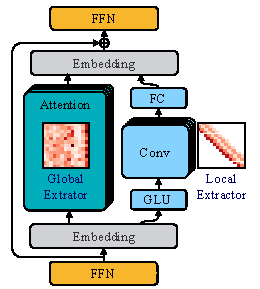
\includegraphics[width=.48\textwidth]{literature/imgs/ext-2-lite-transformer.pdf}
    \caption{Lite Transformer block \cite{wu2020lite}}
    \label{fig:ext-2-lite-transformer}
\end{wrapfigure}

Figure \ref{fig:ext-2-lite-transformer} displays the structure of the proposed Long-Short Range Attention that one group of heads models the local context with convolution while another group focuses on the long-distance relationship with full attention.
This method takes advantage of the convolution that is good at capturing local features with small calculation resource required while using the attention mechanism that is good at long-distance.
It concludes that using self-attention only overemphasises the local features, and it is possible to use another modelling method in Transformer-based models.

\citet{beltagy2020longformer} published Longformer model, another optimised Transformer-based model, almost at the same time in April 2020, which also pointed out that the self-attention mechanism has limitations when targeting long sequences, depicted in Figure \ref{fig:ext-longformer} (a).

\begin{figure}[!ht]
    \centering
    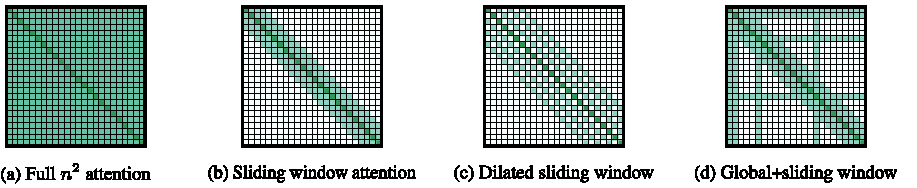
\includegraphics[width=\textwidth]{literature/imgs/ext-longformer.pdf}
    \caption{Full self-attention and attention patterns proposed in Longformer \cite{beltagy2020longformer}}
    \label{fig:ext-longformer}
\end{figure}

In full $n^2$ attention, the time and space complexity are all increased quadratically with the sequence length $n$, because the Queries at each location needs to pay attention to Keys at each location.
An idea proposed in Longformer uses three different attention patterns to build a sparse attention matrix rather than a complete attention matrix.

The first method is to use a fixed-size sliding window that goes through each token to calculate local attention (Figure \ref{fig:ext-longformer} (b)).
In this way, each token only needs to pay attention to the tokens within the sliding window size $w$.
Although it undermines some long-distance attention ability, it greatly reduces the amount of calculation required to $O(w \times n)$ in terms of computation complexity.

The second method is using a dilated sliding window (Figure \ref{fig:ext-longformer} (c)) in attention to create larger receptive field, which is analogous to using dilated CNN in atrous convolution.
This method also has computation complexity $O(w \times n)$, but expands the receptive field size to $l \times d \times w$, where $l$ denotes the number of layers in Transformer, and $d$ for dilation rate.

The third method is designed specifically to handle tasks that require global attention (Figure \ref{fig:ext-longformer} (d)), such as text classification and question answering.
For example, in classification tasks, a $[CLS]$ token is added to the head of all tokens with a global attention mark, indicating that the token requires global attention computation on all other tokens in the matrix.
And in question answering tasks, the question and document are concatenated together and input to the model.
Then mark the entire question sentence to calculate the global attention, and find the answer in the document.

In a recently published paper, \citet{mehta2020delight} summarised three previously extensively studied methods to optimise the efficiency (higher performance with fewer parameters) on Transformer-based models, which are:

\begin{enumerate}
    \item Improving transformers
    \begin{enumerate}
        \item Improving the usage of self-attention on long sequences. (Longformer proposed by \citet{beltagy2020longformer})
        \item Explaining multi-head attention and possible redundant representations.
        \item Learning better representations, e.g. using convolution (Lite Transformer proposed by \citet{wu2020lite})
    \end{enumerate}
    \item Model scaling: a common way to improve the performance of deep models. \\
    Increasing dimensions in width-wise scaling and stacking more blocks in depth-wise scaling, which is analogous to the model scaling ideas in EfficientNet.
    \item Improving sequence models
    \begin{enumerate}
        \item Using better token-level representation.
        \item Using model compression, pruning and distillation.
    \end{enumerate}
\end{enumerate}
